\chapter{Project Requirements}

\section{Functional and Nonfunctional Requirements}

In the development of any software application, defining clear and comprehensive requirements is essential to guide the design and development process. These requirements are typically categorized into two main types: functional and non-functional requirements. The following sections will dive into what, exactly, these two types of requirements entail, and what requirements have been identified for my project.

\subsection{Functional Requirements}

Functional requirements describe the specific features and functionalities that an application must possess to meet the needs of its users. For my application, which focuses on OIT and aims to provide a comprehensive and user-friendly experience, several functional requirements have been identified.

First, I've identified the following as critical functional requirements. Critical requirements are the highest priority and must-have features or functionalities. These are non-negotiable elements that are essential for the core functionality and success of the application. Failure to implement critical requirements would severely impact the application's usability or safety.

\begin{itemize}
    \item \textbf{Integration with Apple Health App:} The application will seamlessly integrate with the Apple Health app, allowing it to retrieve and display health metrics relevant to OIT, such as exercise and heart rate.
    \item \textbf{Data Logging and Tracking:} Users will be able to log their daily OIT doses and associated symptoms. The app will also enable users to input and track their treatment progress over time.
\end{itemize}

Next, I've identified the following as necessary functional requirements, or important features and attributes that are required for the software to function effectively and provide a satisfactory user experience. While not as vital as critical requirements, necessary requirements are still essential for the software to fulfill its intended purpose and meet user expectations.
They are the second-highest priority and are addressed immediately after critical requirements, and are crucial for the software's overall functionality and user satisfaction.

\begin{itemize}
    \item \textbf{Data Visualization:} To assist users in understanding their progress, the application will provide graphical representations of long-term trends in OIT progress. These charts and graphs will be interactive and easy to interpret.
    \item \textbf{Data Sharing:} Users will have the capability to securely share their OIT data with healthcare providers through Apple Health, ensuring efficient communication between patients and professionals.
\end{itemize}

Finally, I've identified the following optional requirements. Also known as ``nice-to-have" or ``enhancement" features, these are functionalities or attributes that are not essential for the core functionality of the software and are the lowest priority to implement.

\begin{itemize}
    \item \textbf{Educational Resources:} The application will offer educational content on essential topics like anaphylaxis and oral immunotherapy, including articles and other educational materials to empower users with knowledge.
    \item \textbf{Notifications:} The application will send reminders and alerts to users for taking their doses and logging symptoms, with customizable notification settings to accommodate individual preferences.
\end{itemize}

\subsection{Nonfunctional Requirements}

Nonfunctional requirements, on the other hand, focus on the qualities or attributes of the application that enhance its overall performance and user experience. These requirements ensure the application functions effectively and efficiently while adhering to certain standards and guidelines. 

The following are critical nonfunctional requirements that have been identified for my application. These are the highest priority nonfunctional requirements to implement, and will thus be implemented first.

\begin{itemize}
    \item \textbf{Compliance:} Adherence to Apple's App Store guidelines and healthcare data privacy regulations, such as HIPAA, is crucial to avoid legal and reputational risks.
    \item \textbf{Compatibility:} The application must be compatible with a wide range of iPhone models and iOS versions, optimizing it for different screen sizes and resolutions.
    \item \textbf{User Interface (UI) and User Experience (UX):} An intuitive, user-friendly interface with a consistent and aesthetically pleasing design is imperative to enhance user satisfaction.
\end{itemize}

Next, the necessary nonfunctional requirements are as follows.

\begin{itemize}
    \item \textbf{Reliability:} The app should function reliably without frequent crashes or errors. Implementing error handling and reporting mechanisms helps ensure a seamless user experience.
    \item \textbf{Performance:} The application must be responsive, providing a smooth user experience with minimized load times for data and visual elements to ensure users are not kept waiting.
\end{itemize}

Finally, the optional nonfunctional requirements are listed below.

\begin{itemize}
    \item \textbf{Accessibility:} Accessibility for users with disabilities is a non-negotiable requirement, necessitating compliance with accessibility guidelines and standards.
    \item \textbf{Scalability:} The application's architecture could be designed to accommodate potential growth in the user base, ensuring it can handle increased data and user loads gracefully.
\end{itemize}

\section{Use Cases}

After defining the nonfunctional and functional requirements, the next natural step is a comprehensive analysis and visualization of the system's functionalities. This section delves into the Use Case Tables and Unified Modeling Language (UML) diagrams that serve as the blueprint for my envisioned app. These diagrams are instrumental in illustrating various interactions between users and the application, offering a systematic representation of the app's behavior, structure, and relationships. The Use Case Tables and UML diagrams dive into the specific scenarios in which users engage with the application, outlining the goals and interactions within each use case.

% \begin{table}[ht]
\centering
\caption{Use Case 01: Initial App Onboarding}

\hspace{1em}
\renewcommand{\arraystretch}{1.7}

\begin{tabular}{|c|p{2em}|p{14cm}|}
\hline
\textbf{Dependencies} & \multicolumn{2}{|p{14cm}|}{User has never opened the app before} \\ 
\hline
\textbf{Description} & \multicolumn{2}{|p{14cm}|}{The system will behave in the following use case when the user initially opens the app.} \\
\hline
\textbf{Precondition} & \multicolumn{2}{|p{14cm}|}{The user has downloaded the app from the app store and goes to use it.} \\
\hline
\multirow{7}{4em}{\textbf{Ordinary Sequence}} & \textbf{Step} & \textbf{Action} \\
& 1 & Application displays a screen, with a button to get started \\
& 2 & User taps the “Get Started” button \\
& 3 & Application displays a screen with basic information for the user to fill out: Name, Birthdate, Allergens, Preferences, Share Data with Apple Health, Protect Application with FaceID \\
& 4 & User fills out the necessary information: Name, Birthdate, Allergens, Preferences, Share Data with Apple Health, Protect Application with FaceID \\
& 5 & User taps “Get Started” button \\
& 6 & Application saves information, sets a flag that the user has opened the application before, and then displays the tabbed application \\
\hline
\textbf{Postcondition} & \multicolumn{2}{|p{14cm}|}{The user will be able to use the application.} \\
\hline
\textbf{Exceptions} & 6 & If the user hasn’t filled out all of the necessary information, then an alert will be displayed to complete the information, and the user won’t be able to proceed until everything’s completed. \\
\hline
\textbf{Comments} & \multicolumn{2}{|p{14cm}|}{The information entered here will be displayed in the profile section of the app and will be editable.} \\
\hline
\end{tabular}
\end{table}

% \begin{table}[ht]
\centering
\caption{Use Case 02: Sharing Data with Apple Health}

\hspace{1em}
\renewcommand{\arraystretch}{1.7}

\begin{tabular}{|c|p{2em}|p{14cm}|}
\hline
\textbf{Dependencies} & \multicolumn{2}{|p{14cm}|}{User hasn’t enabled sharing data with Apple health yet} \\ 
\hline
\textbf{Description} & \multicolumn{2}{|p{14cm}|}{The system will behave in the following use case when the user enables sharing data with Apple health.} \\
\hline
\textbf{Precondition} & \multicolumn{2}{|p{14cm}|}{The user is going through the setup page.} \\
\hline
\multirow{6}{4em}{\textbf{Ordinary Sequence}} & \textbf{Step} & \textbf{Action} \\
& 1 & Application displays a screen with basic information for the user to fill out: Name, Birthdate, Allergens, Preferences, Share Data with Apple Health, Protect Application with FaceID \\
& 2 & User taps the “Share Data with Apple Health” toggle, toggling it on \\
& 3 & Application displays a pop up sheet, asking the user if they would like to share data with the Apple Health app. It will list out every symptom / thing that it will be reading from Apple Health / writing to Apple Health. \\
& 4 & User goes through all of the options and decides whether or not they would like to share that data, tapping on the toggles. \\
& 5 & User taps “Done” \\
\hline
\textbf{Postcondition} & \multicolumn{2}{|p{14cm}|}{The user will have all of the selected data shared with Apple Health.} \\
\hline
\textbf{Exceptions} & 0 & If the user has already gone through the onboarding process, they can edit their permissions in the Profile section, and then follow the ordinary sequence. \\
\hline
\textbf{Comments} & \multicolumn{2}{|p{14cm}|}{The user doesn’t have to select all of the categories, if they’re uncomfortable sharing that information.} \\
\hline
\end{tabular}
\end{table}


\begin{table} [H]
    \centering
    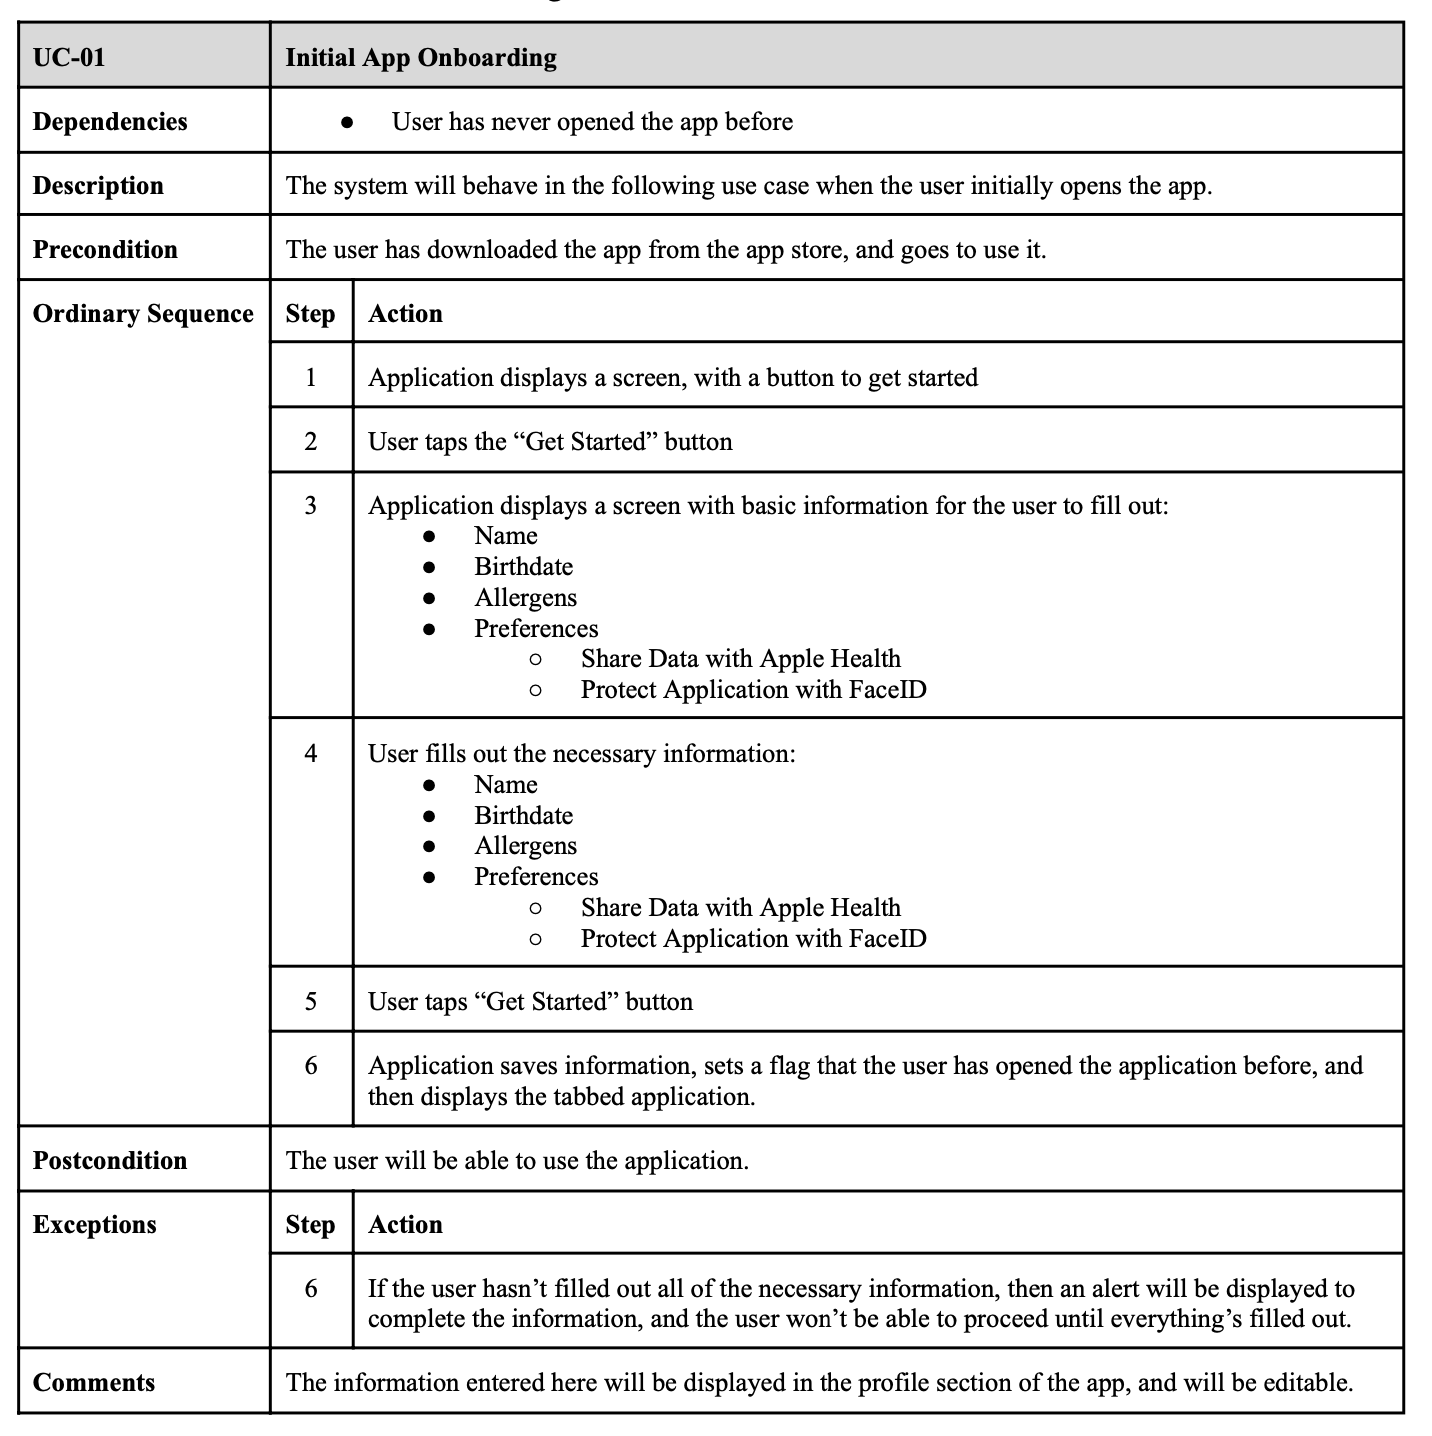
\includegraphics[width=1\linewidth]{thesis//chapters//images/uc-01.png}
    \caption{Use Case 01: Initial App Onboarding}
    \label{fig:uc01-table}
\end{table}

\begin{table} [H]
    \centering
    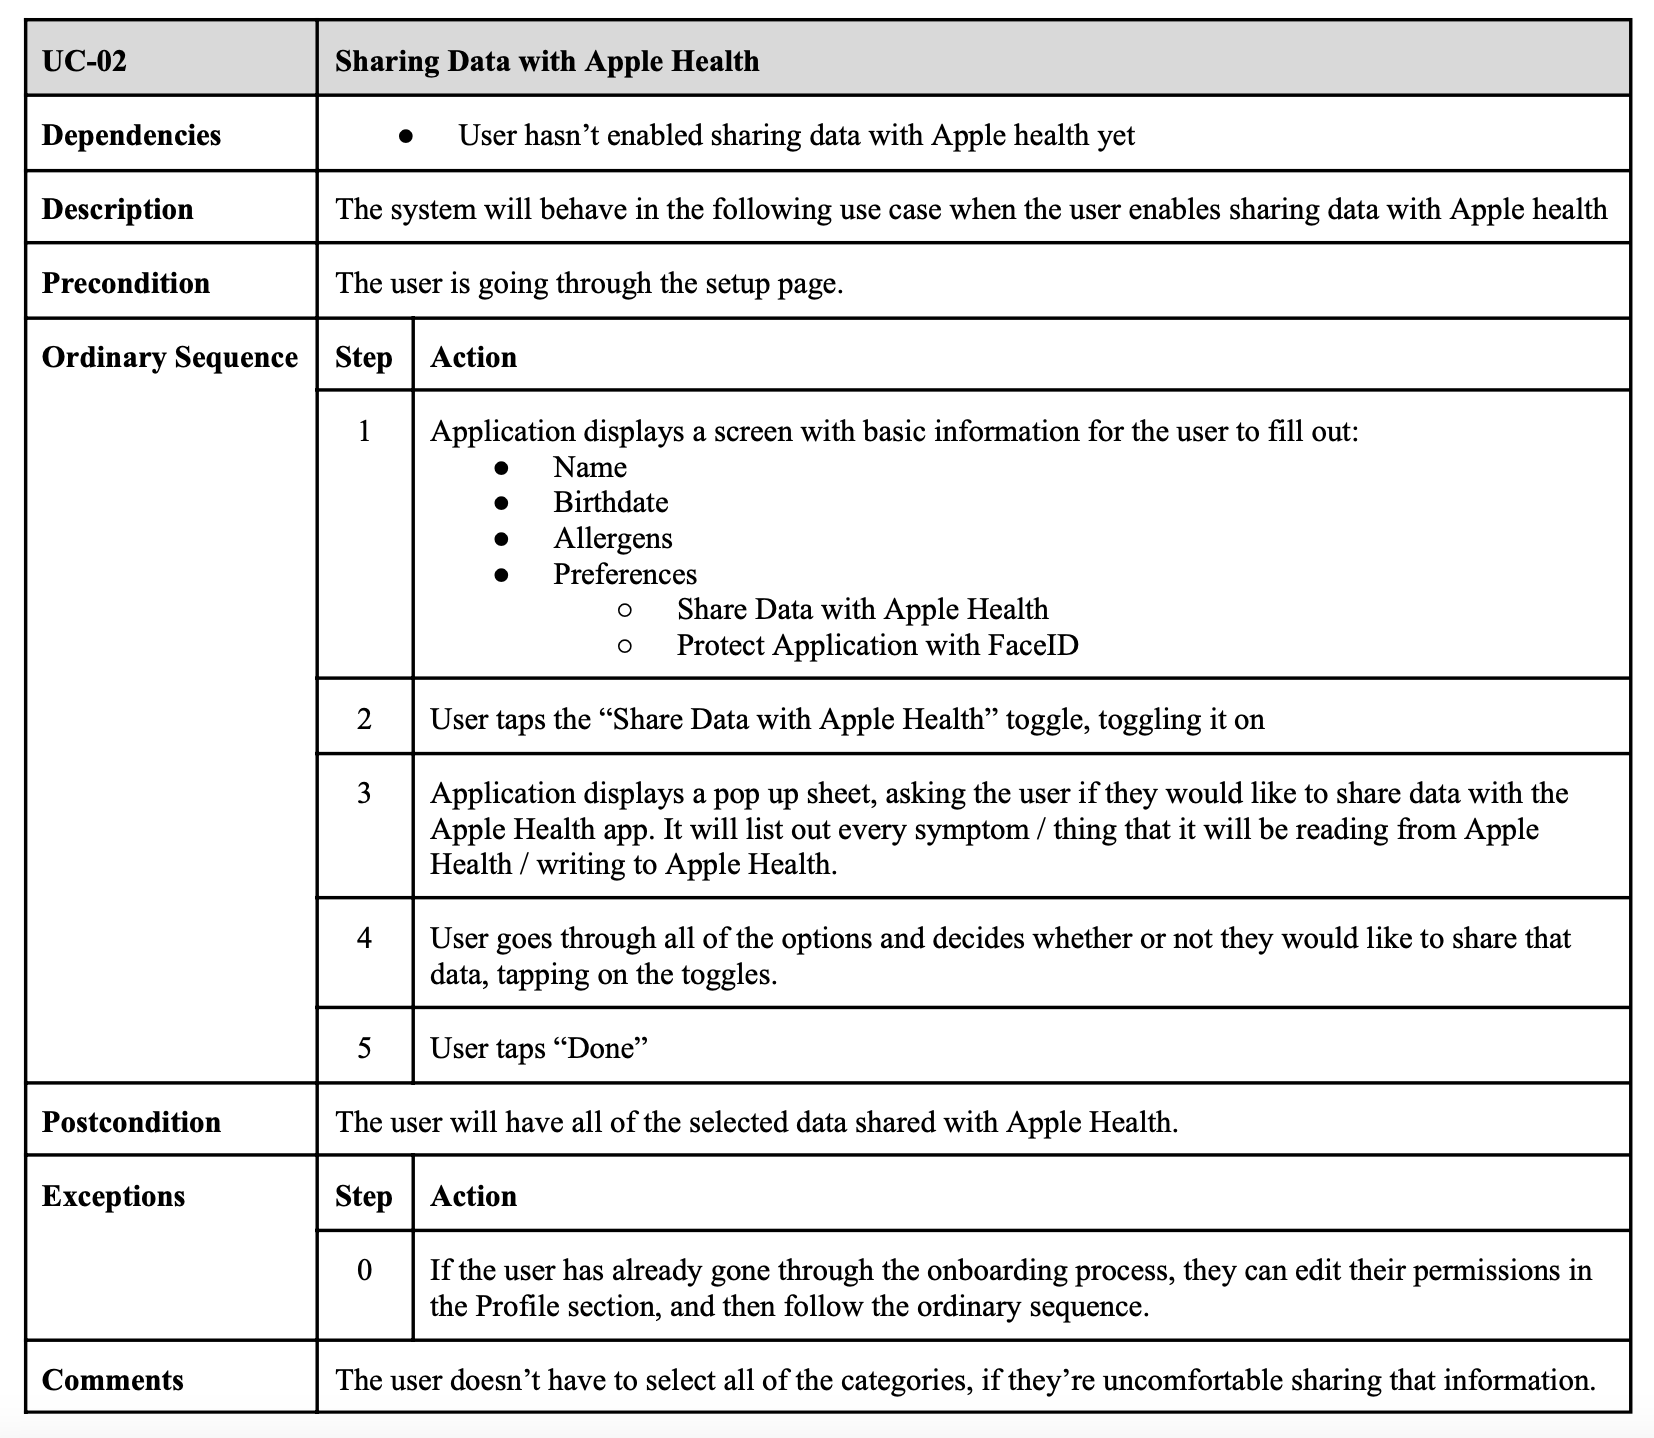
\includegraphics[width=1\linewidth]{thesis//chapters//images/uc-02.png}
    \caption{Use Case 02: Sharing Data with Apple Health}
    \label{fig:uc02-table}
\end{table}

\begin{figure} [H]
    \centering
    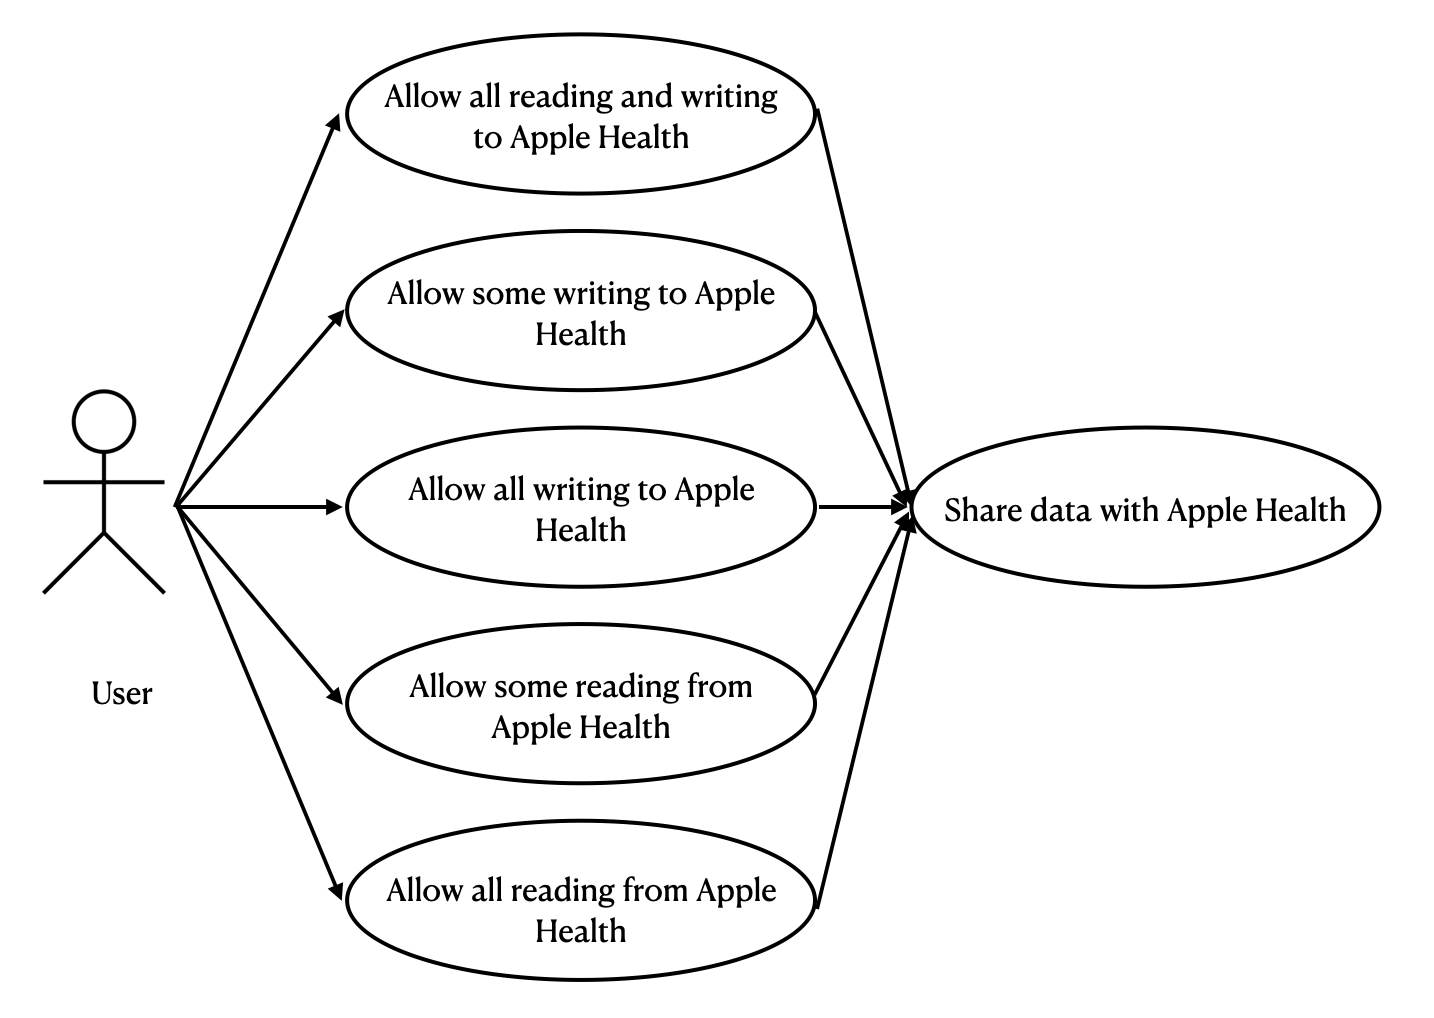
\includegraphics[width=0.75\linewidth]{thesis//chapters//images/uc-02-visual.png}
    \caption{Use Case 02: Visual Diagram}
    \label{fig:uc02-visual-diagram}
\end{figure}

\begin{table} [H]
    \centering
    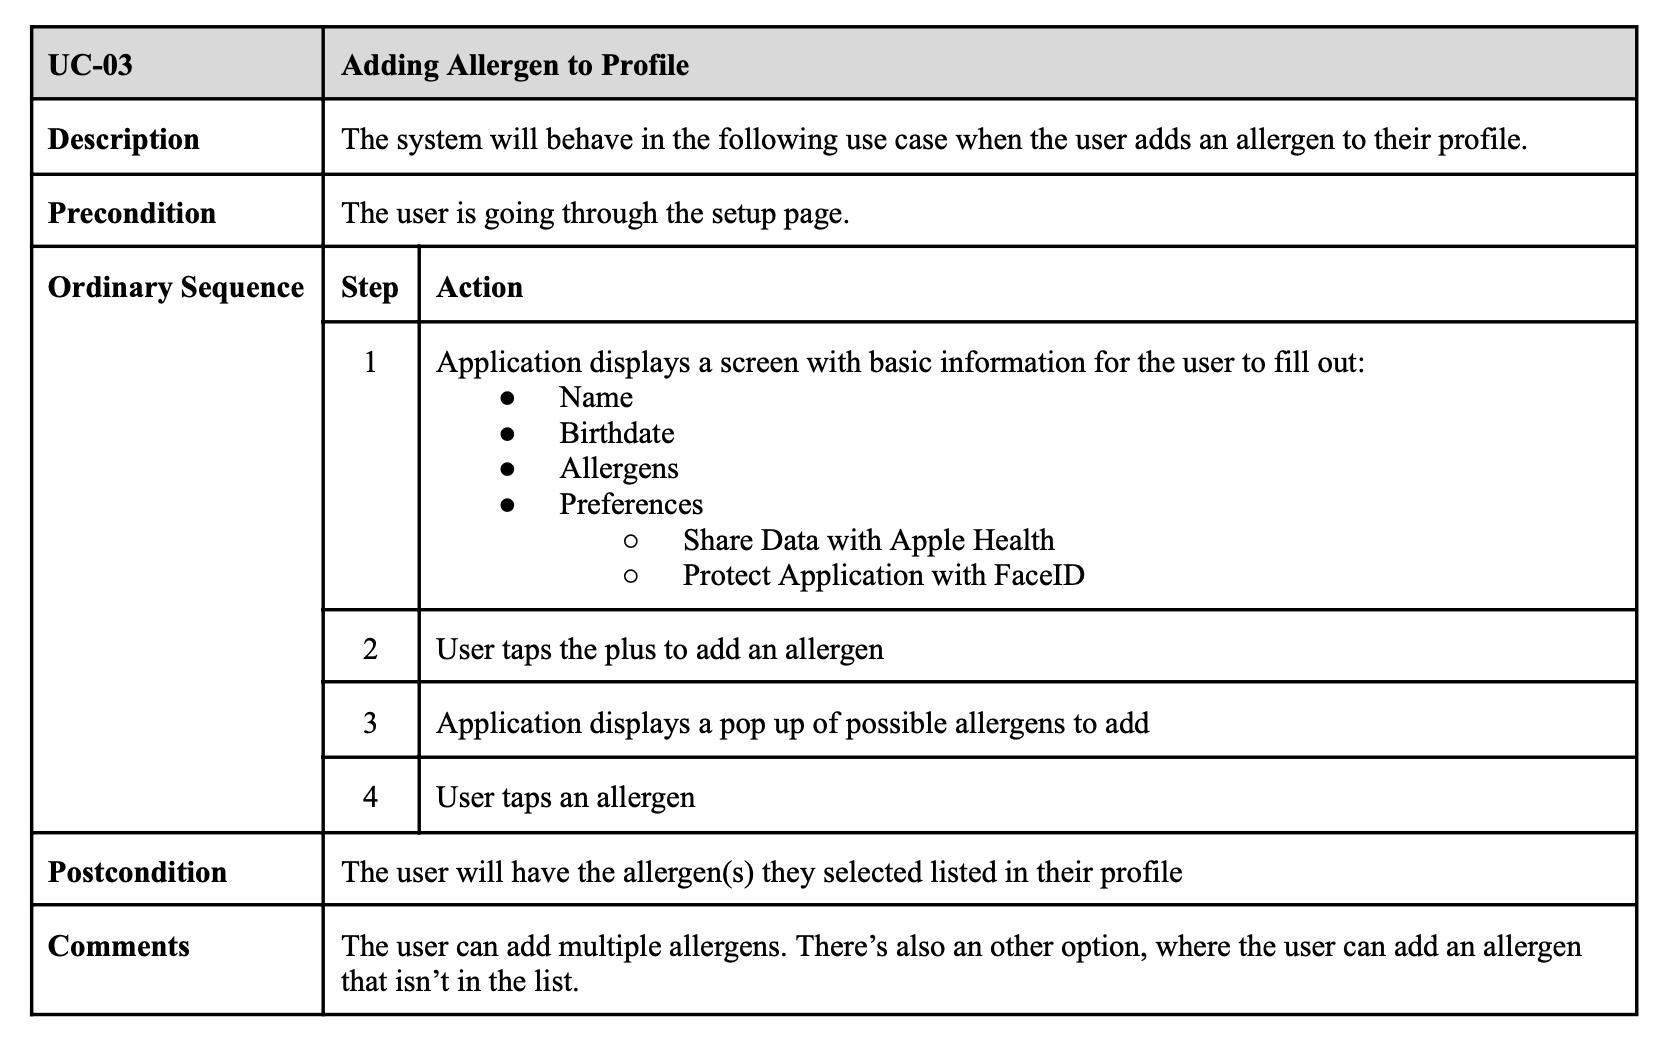
\includegraphics[width=1\linewidth]{thesis//chapters//images/uc-03.png}
    \caption{Use Case 03: Adding Allergen to Profile}
    \label{fig:uc03-table}
\end{table}

\begin{figure} [H]
    \centering
    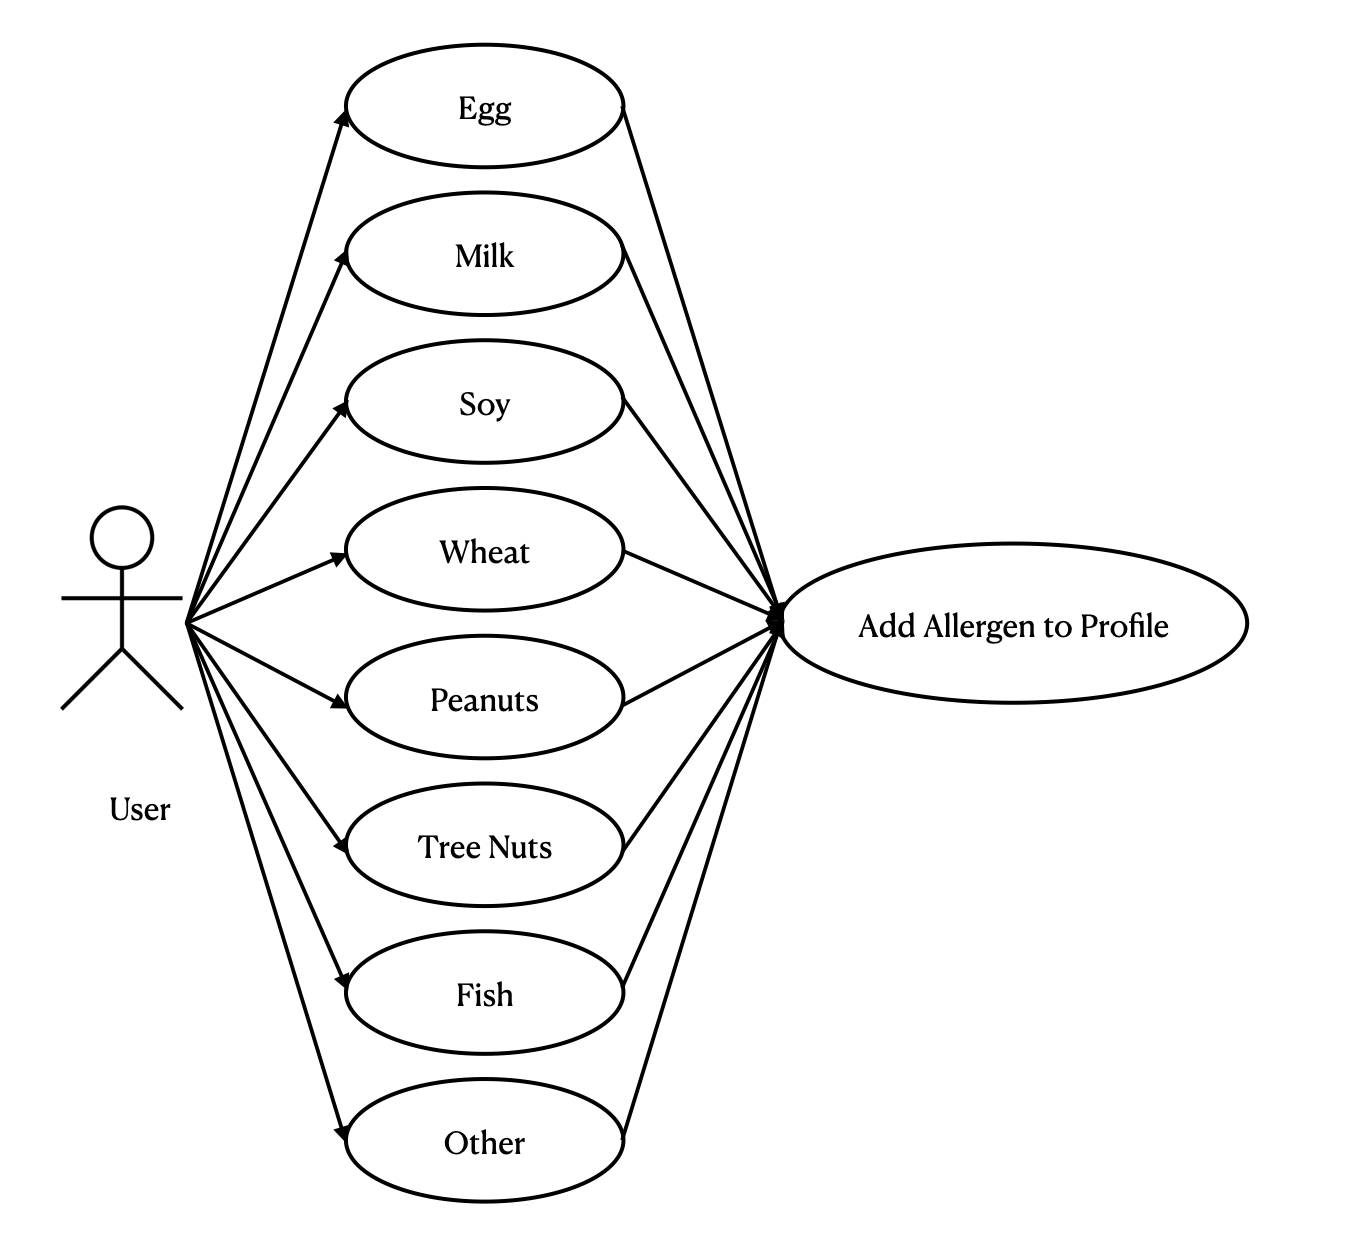
\includegraphics[width=0.75\linewidth]{thesis//chapters//images/uc-03-visual.png}
    \caption{Use Case 03: Visual Diagram}
    \label{fig:uc03-visual-diagram}
\end{figure}

\begin{table} [H]
    \centering
    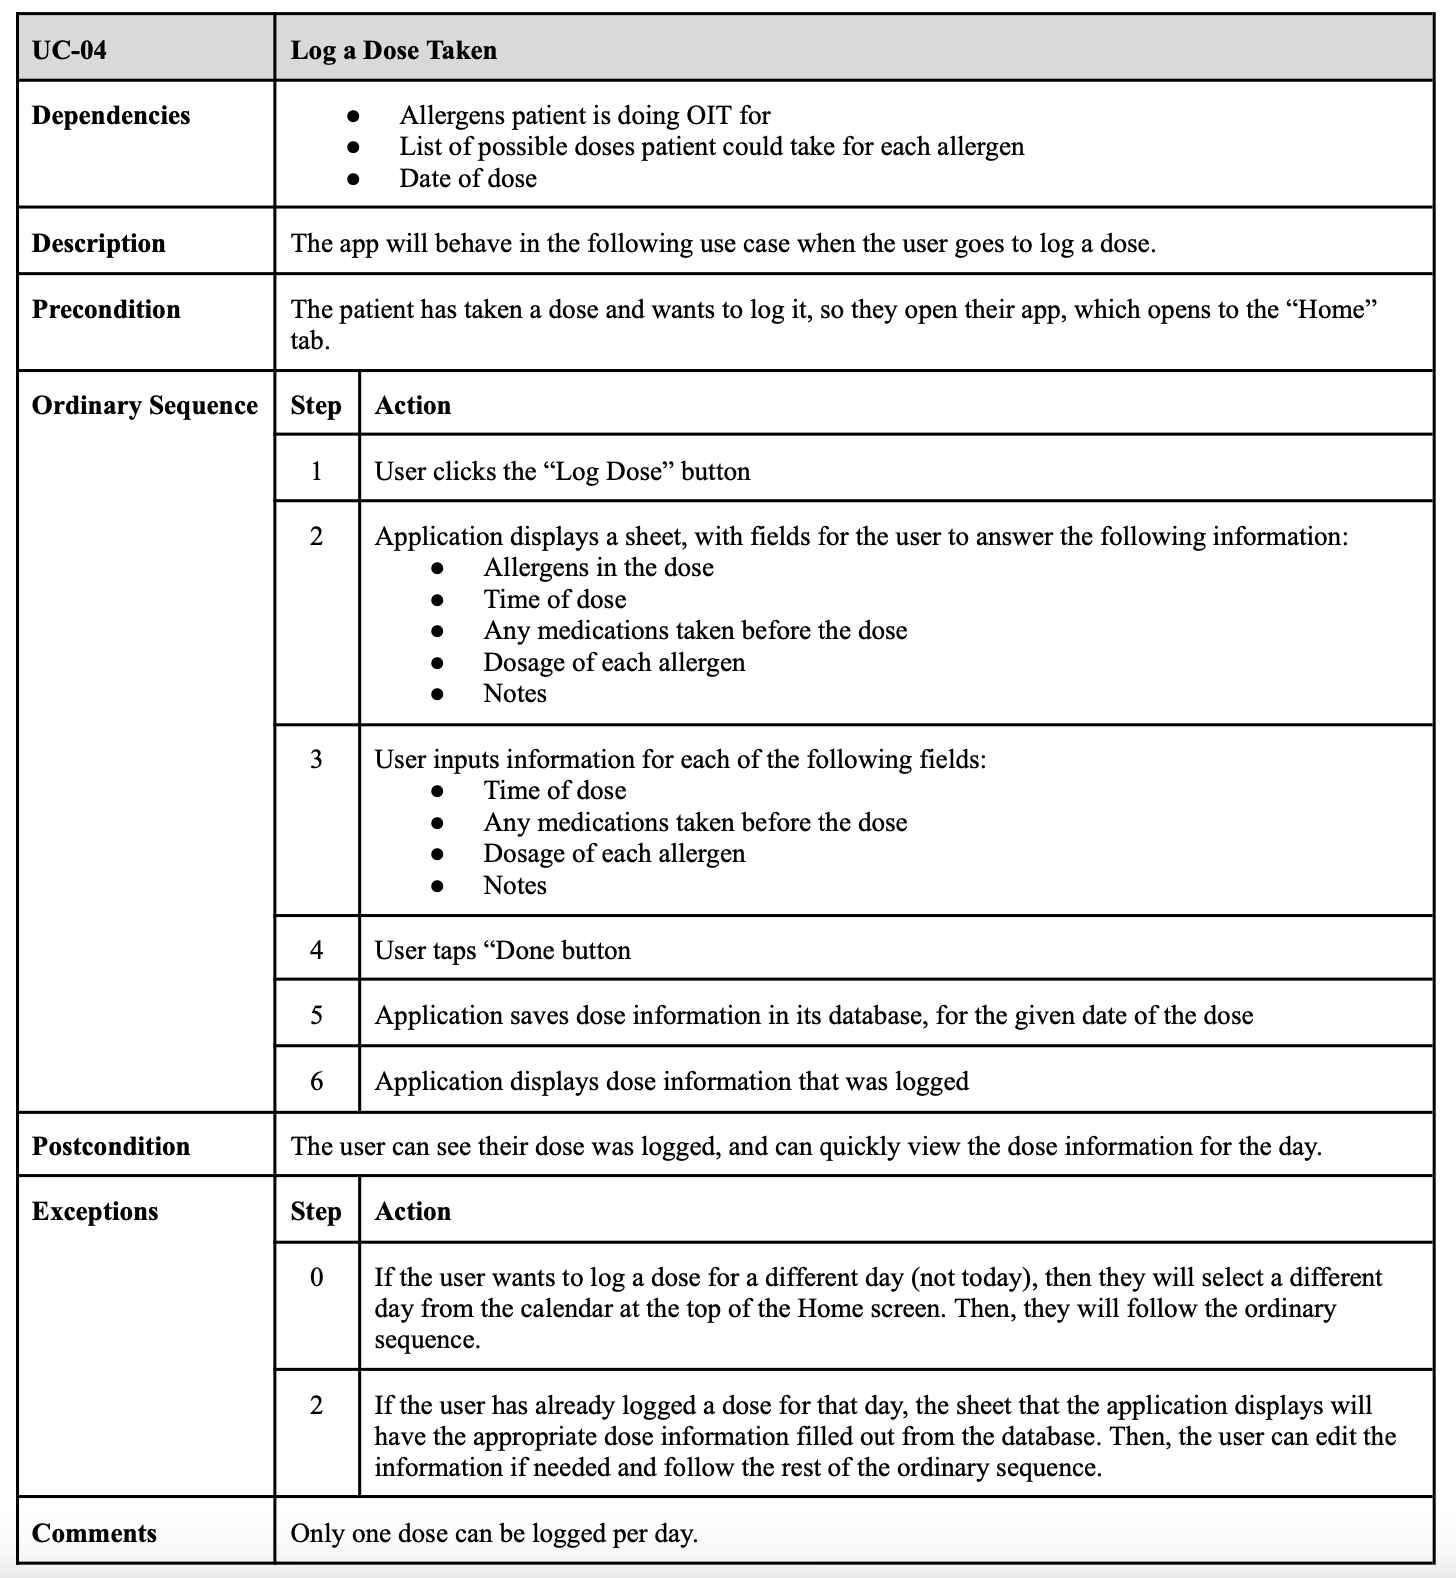
\includegraphics[width=1\linewidth]{thesis//chapters//images/uc-04.png}
    \caption{Use Case 04: Log a Dose Taken}
    \label{fig:uc04-table}
\end{table}

\begin{figure} [H]
    \centering
    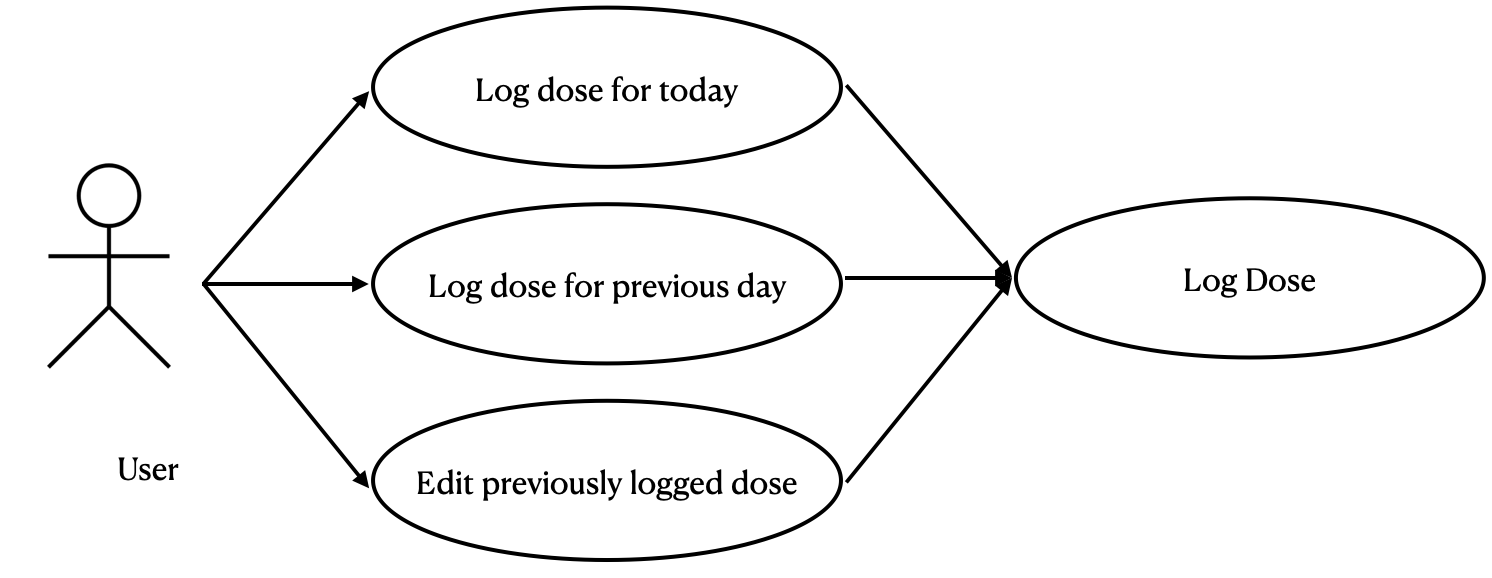
\includegraphics[width=0.75\linewidth]{thesis//chapters//images/uc-04-visual.png}
    \caption{Use Case 04: Visual Diagram}
    \label{fig:uc04-visual-diagram}
\end{figure}

\begin{table} [H]
    \centering
    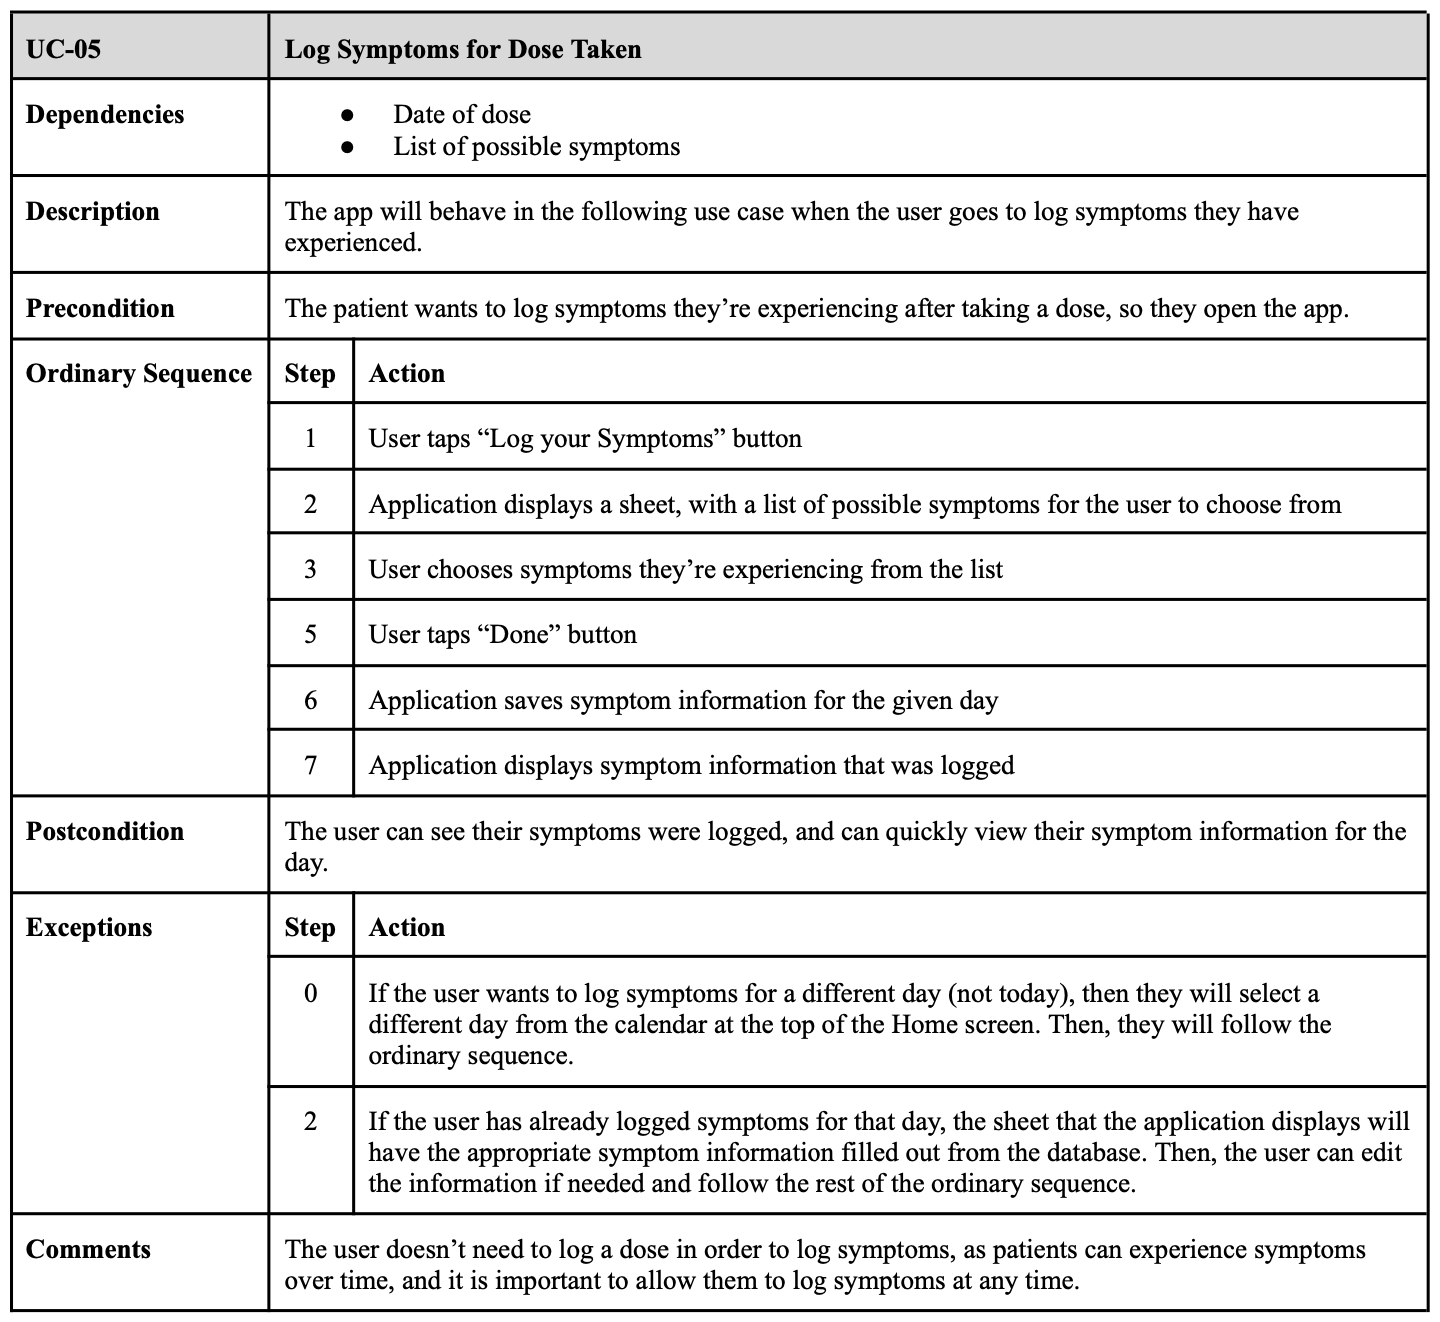
\includegraphics[width=1\linewidth]{uc-05.png}
    \caption{Use Case 05: Log Symptoms for Dose Taken}
    \label{fig:uc05-table}
\end{table}

\begin{figure} [H]
    \centering
    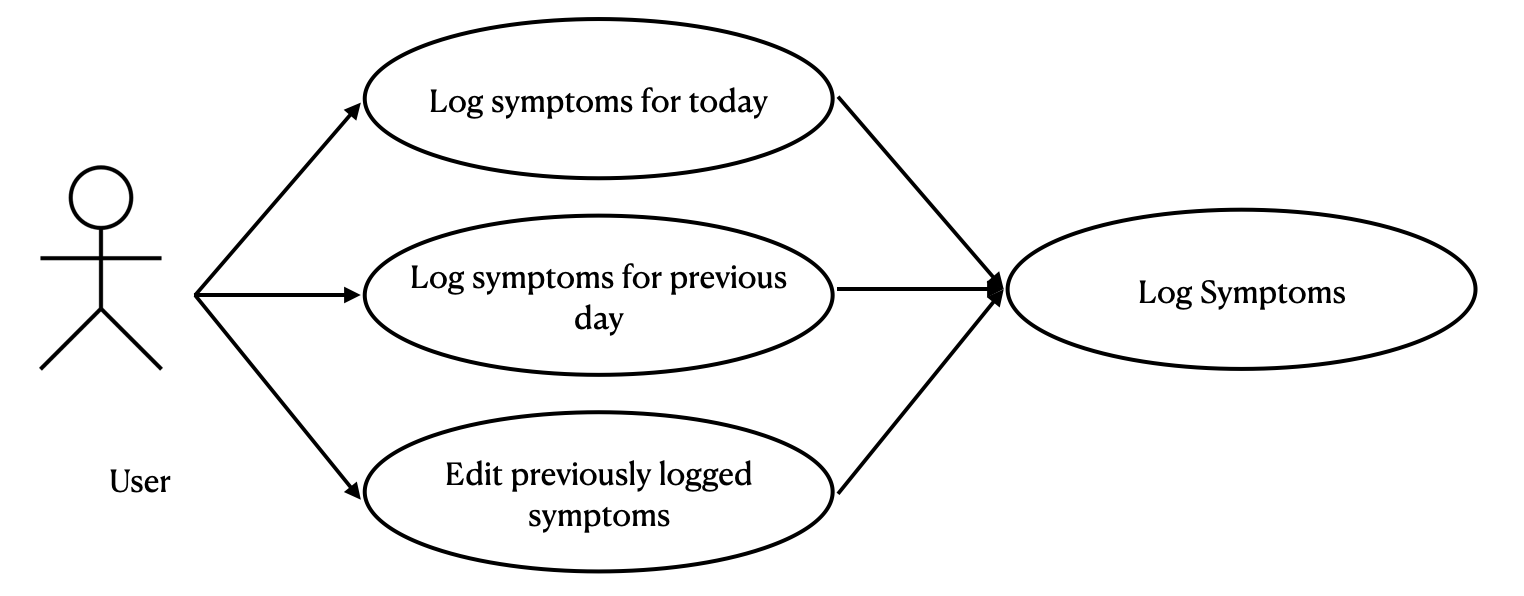
\includegraphics[width=0.75\linewidth]{thesis//chapters//images/uc-05-visual.png}
    \caption{Use Case 05: Visual Diagram}
    \label{fig:uc05-visual-diagram}
\end{figure}

\begin{table} [H]
    \centering
    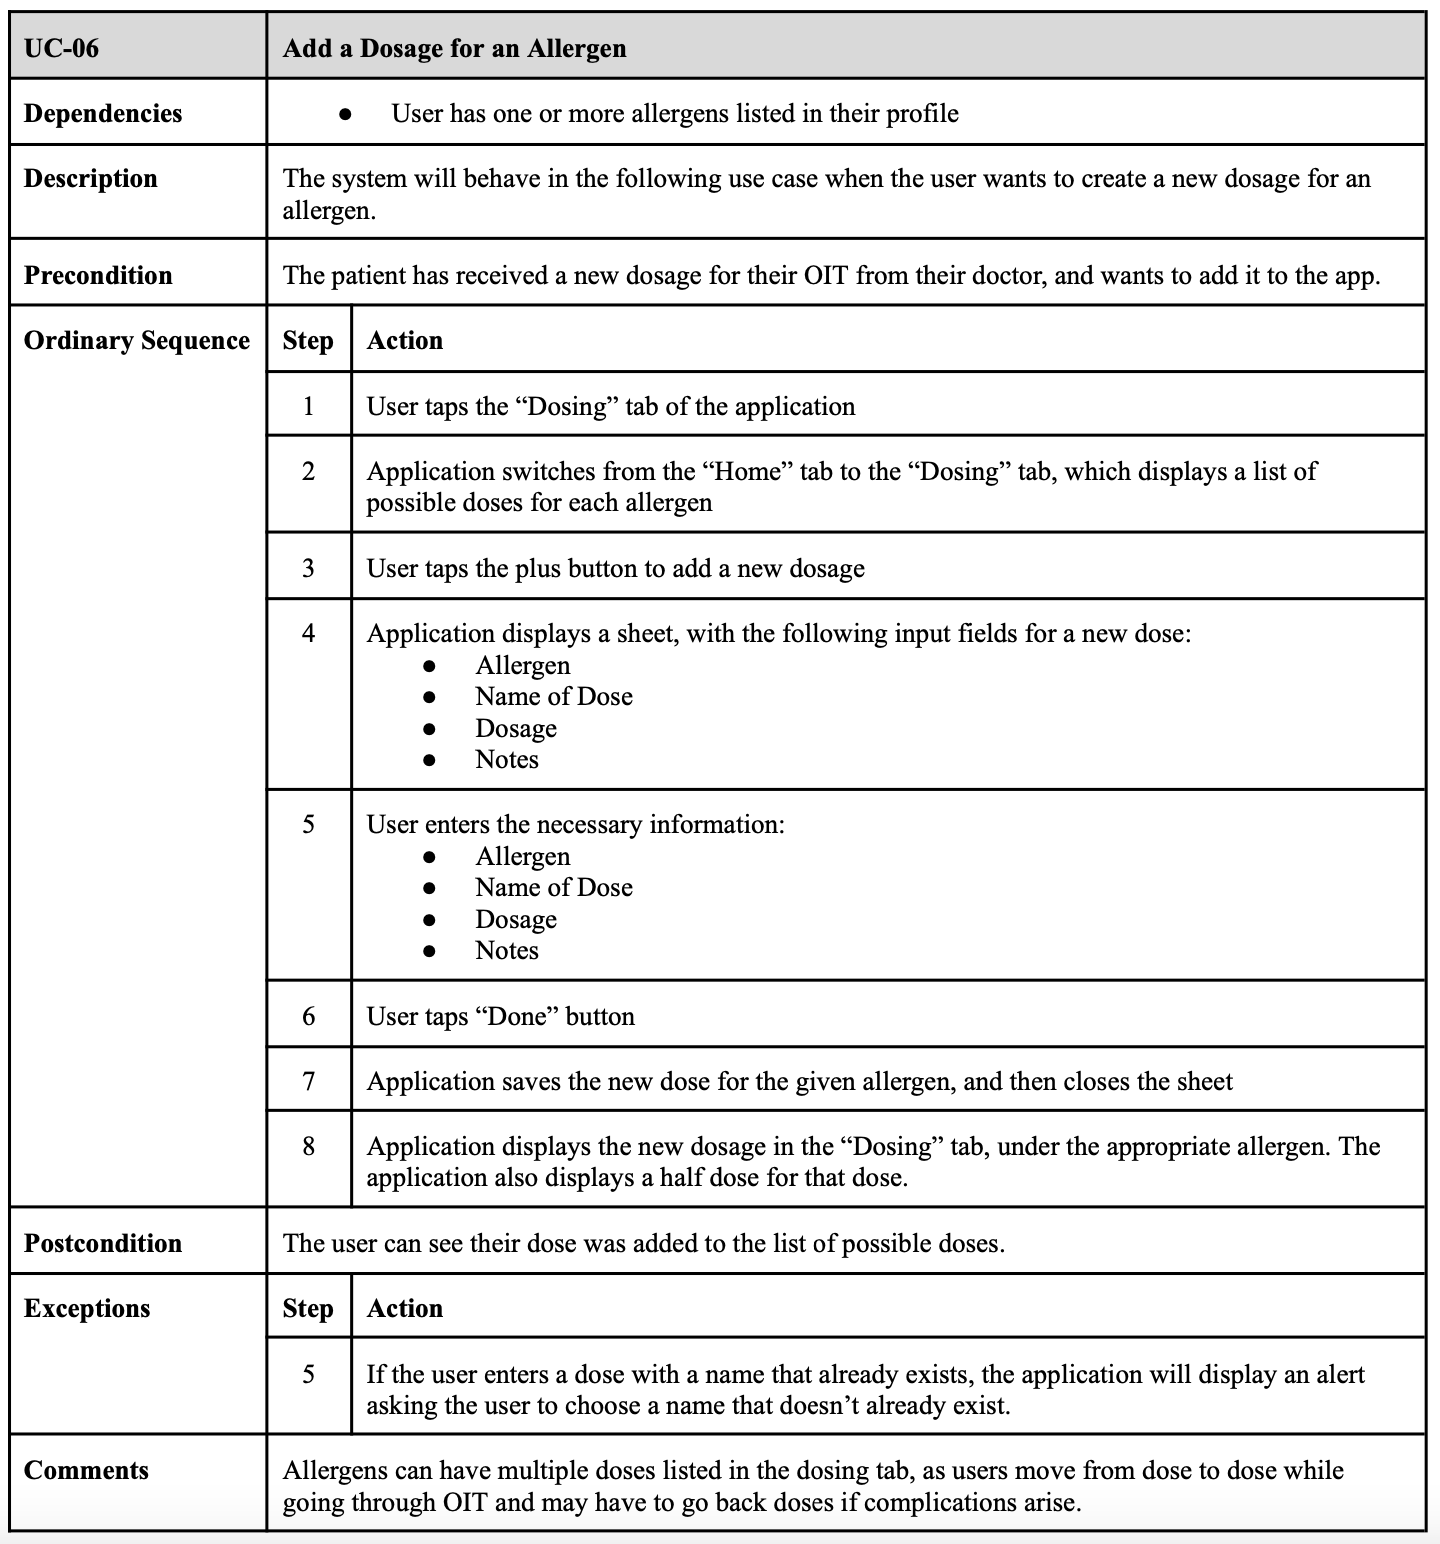
\includegraphics[width=1\linewidth]{uc-06.png}
    \caption{Use Case 06: Add a Dosage for an Allergen}
    \label{fig:uc06-table}
\end{table}

\begin{table} [H]
    \centering
    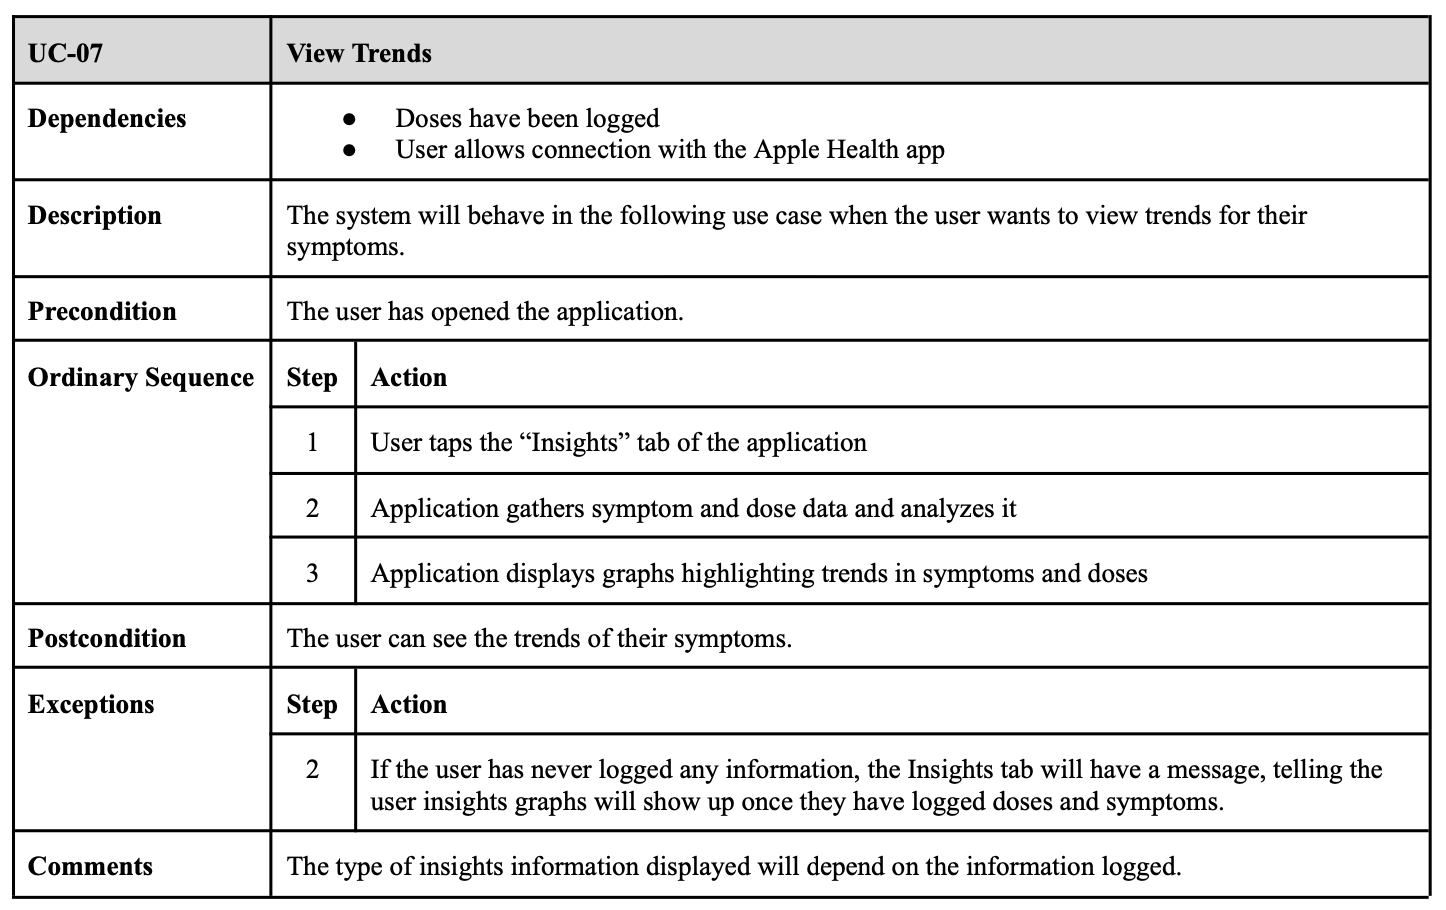
\includegraphics[width=1\linewidth]{thesis//chapters//images/uc-07.png}
    \caption{Use Case 07: View Trends}
    \label{fig:uc07-table}
\end{table}

\begin{table} [H]
    \centering
    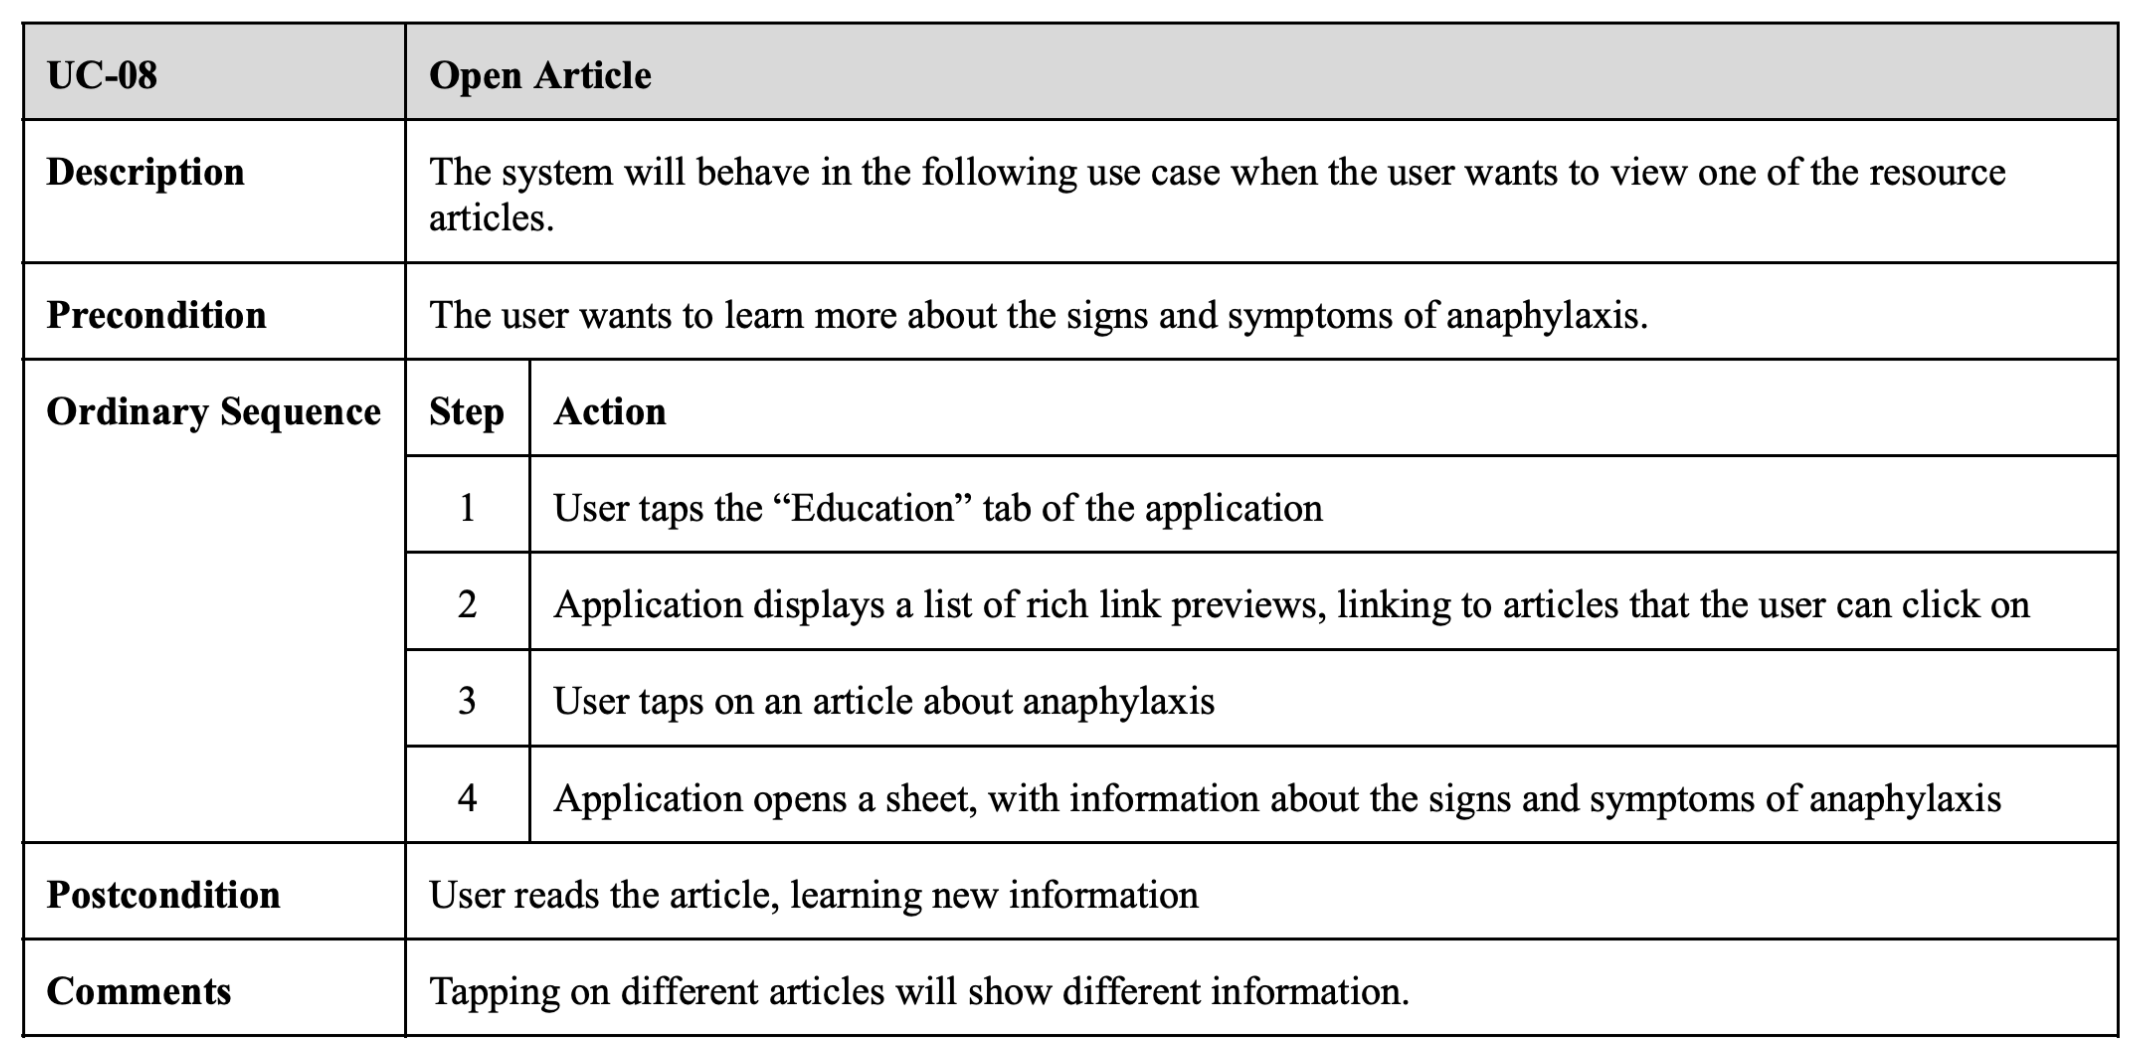
\includegraphics[width=1\linewidth]{thesis//chapters//images/uc-08.png}
    \caption{Use Case 08: Open Article}
    \label{fig:uc08-table}
\end{table}

\begin{table} [H]
    \centering
    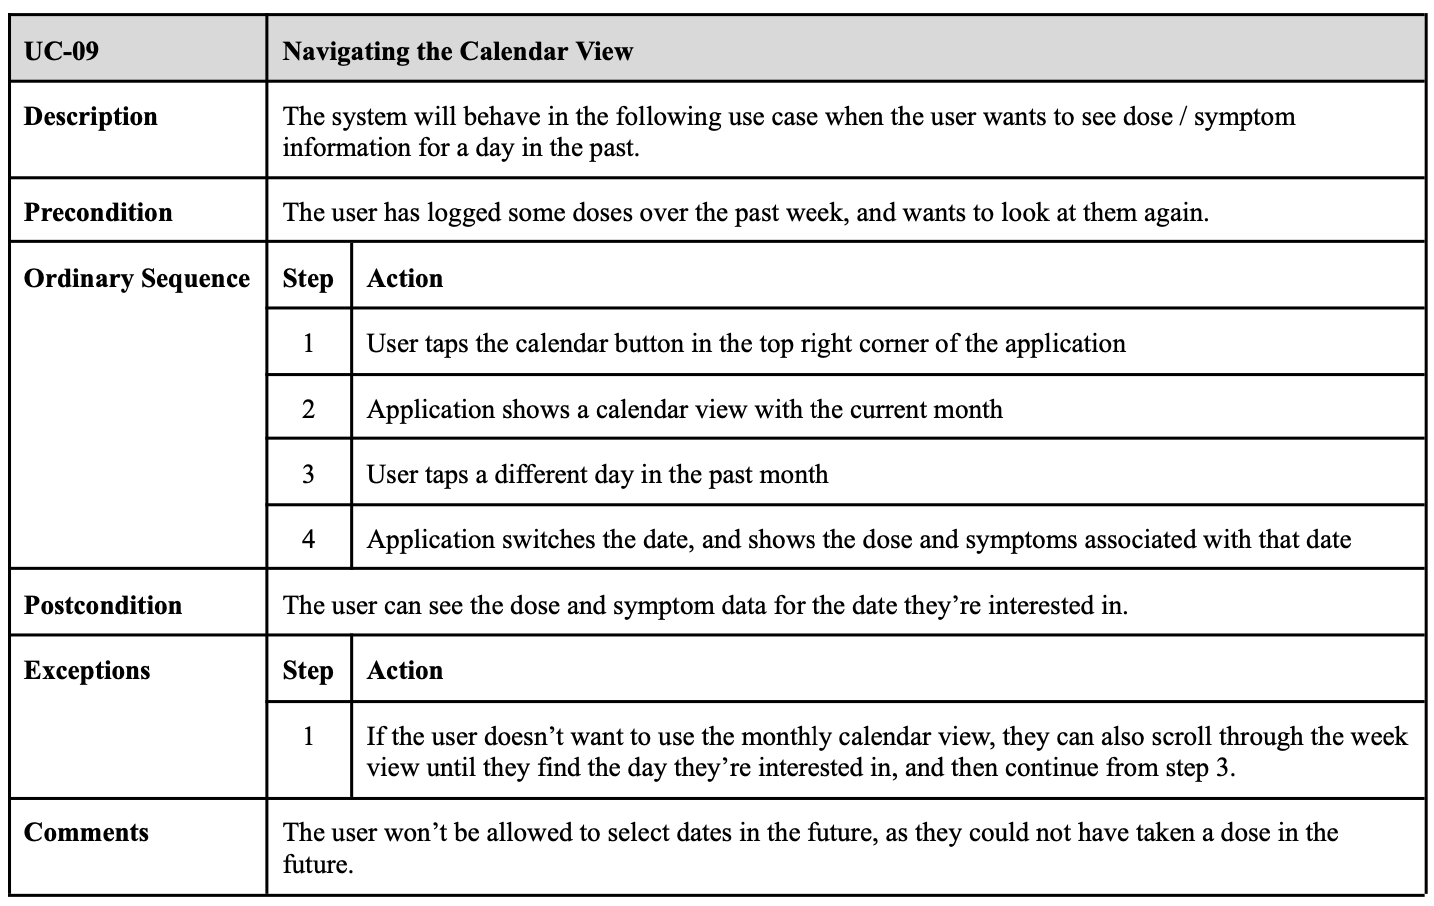
\includegraphics[width=1\linewidth]{thesis//chapters//images/uc-09.png}
    \caption{Use Case 09: Navigating the Calendar View}
    \label{fig:uc09-table}
\end{table}

\begin{figure} [H]
    \centering
    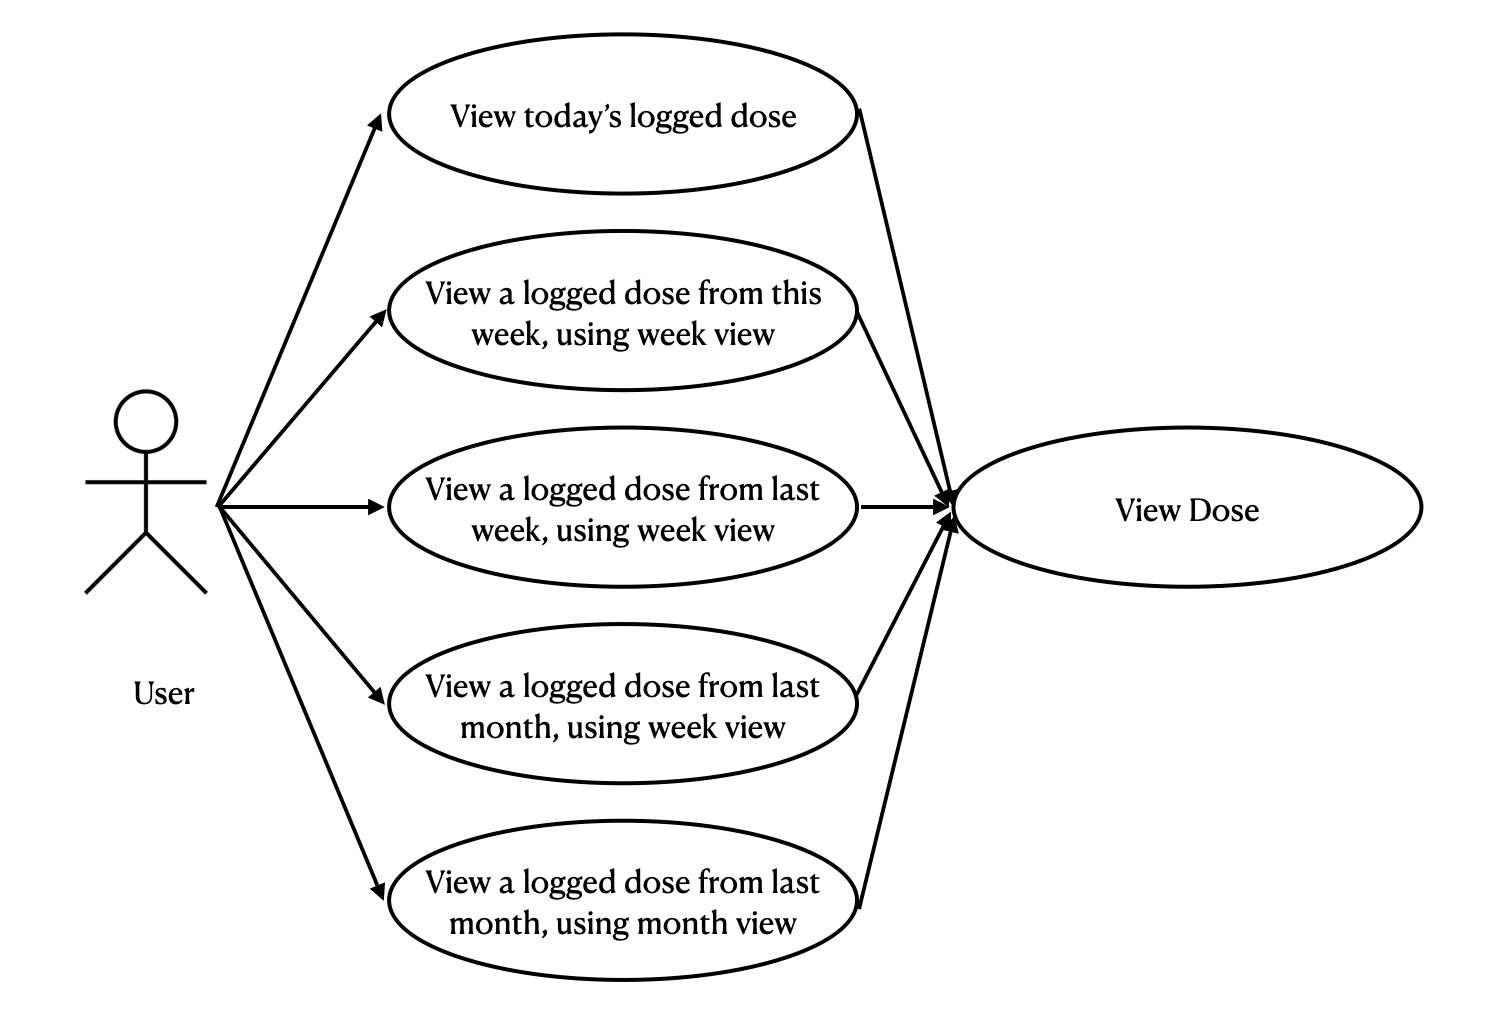
\includegraphics[width=0.75\linewidth]{thesis//chapters//images/uc-09-visual1.png}
    \caption{Use Case 09: Visual Diagram 1}
    \label{fig:uc09-visual-diagram1}
\end{figure}

\begin{figure} [H]
    \centering
    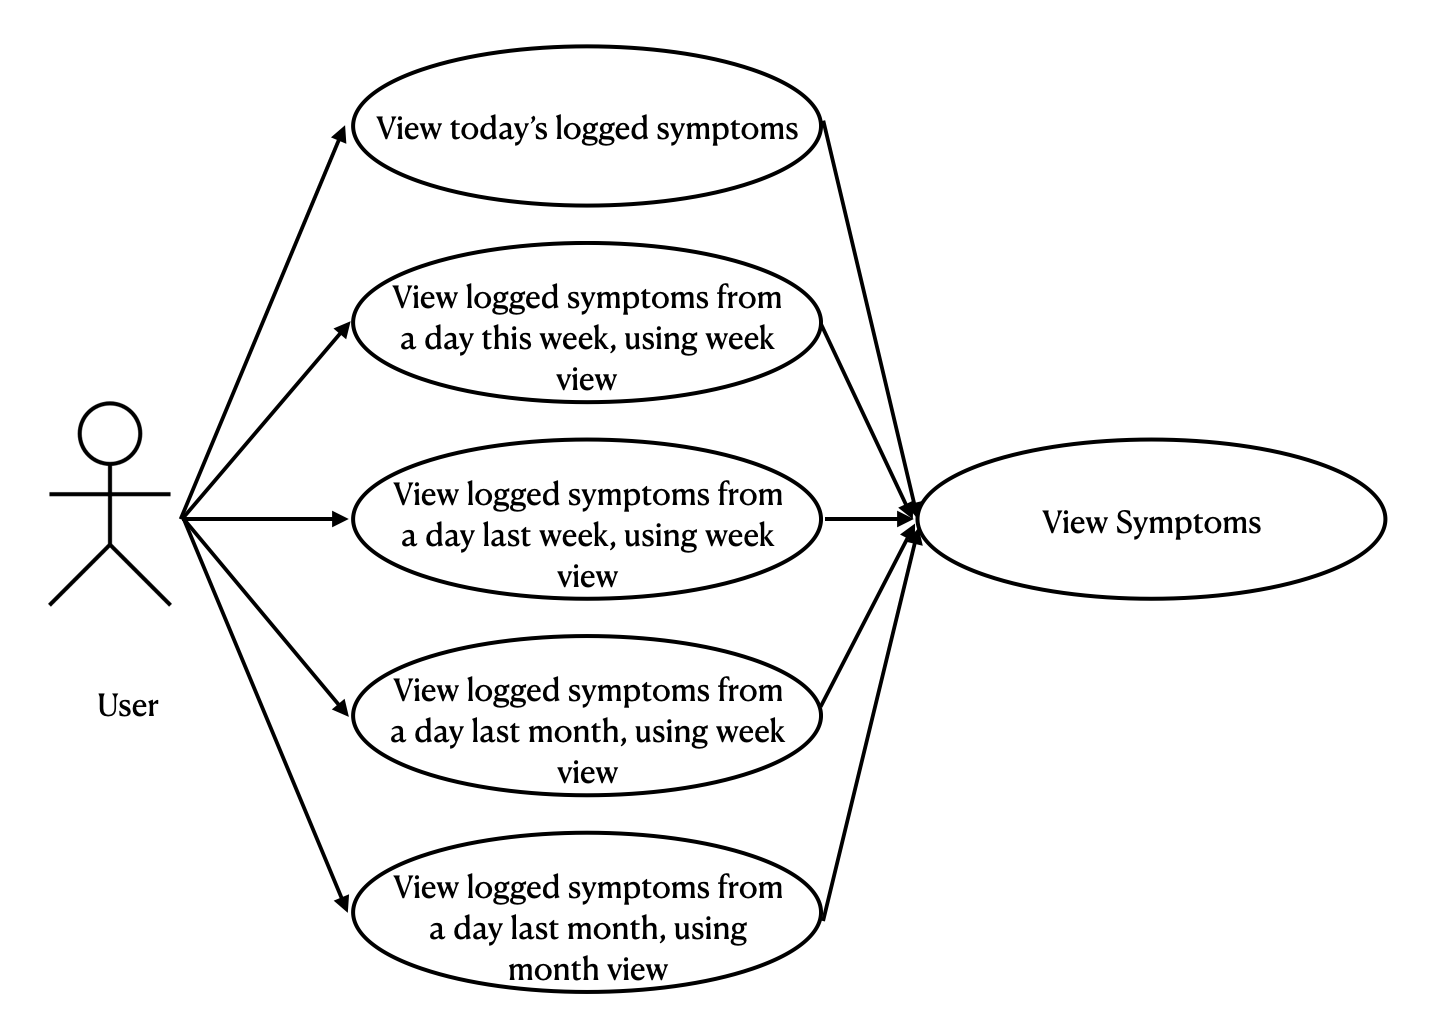
\includegraphics[width=0.75\linewidth]{thesis//chapters//images/uc-09-visual2.png}
    \caption{Use Case 09: Visual Diagram 2}
    \label{fig:uc09-visual-diagram2}
\end{figure}



